\paragraph{Buts}
Le but de cette expérience est de mesurer et d'analyser la force appliquée par une masse à un axe en rotation en faisant varier cette masse, la distance de cette masse au centre de rotation et la vitesse de rotation.
\paragraph{Méthode}
Pour effectuer cette manipulation, le montage ci-dessous a été utilisé:\\
INSERT PHOTO MONTAGE\\
Il est constitué d'une barre métallique attachée en son centre à un dynamomètre électronique captant la force dans l'axe de la barre sus-mentionée.
Cette barre est percée en plusieurs endroits afin d'y placer des masses cylindriques percées en leur centre afin de les glisser le long de l'axe puis de les visser afin de les immobiliser.
Une masse de contre-poids est placée à l'extremité opposée afin de ne pas appliquer trop de force sur l'axe lorsque des masses trop imposantes sont placées en bout de barre.
Un capteur laser est placé le long de la cage afin de de d'indiquer lorsque la barre en rotation coupe de faisceau dans le but de donner la vitesse angulaire $\omega$.

Pour effectuer les mesures, Cassy a été utilisé, un logiciel accompagné d'un boîtier de mesure sur lequel le dynamomètre ainsi que le capteur laser ont été branchés.
Ce boîtier est ensuite relié à un ordinateur sur lequel nous avons pu interagir avec les capteurs pour recevoir leurs mesures (à reformuler).

Pour chaque mesure le procédé suivant a été appliqué.
\begin{enumerate}
    \item Pour chaque changement de masse, vitesse angulaire ou rayon, le mobile a tourné à vide afin de remettre à zéro le capteur de force.
    \item Le masse a été solidement fixée à la distance désirée du centre.
    \item L'axe a été mis en rotation jusqu'à la vitesse angulaire souhaitée, avec quelques secondes d'attente pour être certain que le système se soit stabilisé.
    \item Prise de la mesure grâce à Cassy et ajout de la valeur dans le tableau.
\end{enumerate}

Dans l'objectif d'avoir des mesures les plus précises possibles les masses et leurs vis de fixation ont été précisément mesurées avec un balance ayant une précision au centigramme. Les valeurs suivantes ont été obtenues:
\begin{table}[ht]
    \caption[Mesure des masses]{Mesures des masses}
    \centering
    \begin{tabular}{|l|l|}
	\hline
	Masse théorique [g] & Masse réelle [g]\\
	\hline
	0.050g & $0.0517 \pm 0.01 [g]$\\
	0.075g & $0.0767 \pm 0.01 [g]$\\
	0.100g & $0.1017 \pm 0.01 [g]$\\
	\hline
    \end{tabular}
\end{table}

Les 60 mesures ont donc été efféctuées de cette manière, en variant la vitesse angulaire, ensuite la masse, et finalement le rayon. 

\paragraph{Resultats}
Les resultats bruts sont diponibles en annexe.

Pour l'analyse des données, la consignes de procéder en trois parties a été suivies.
\begin{itemize}
    \item Dans le premier cas, on observe la variation de la force uniquement en fonction du rayon
    \item Dans le second, on continue de regarder la force, mais en faisant varier la masse.
    \item Finalement on donne le rapport entre la force (toujours) et la vitesse angulaire au carré.
\end{itemize}

\subsubsection{Force en fonction du rayon}

\subsubsection{Force en fonction de la masse}

\newpage
\subsubsection{Force en fonction du carré de la vitesse angulaire}

Pour cette partie, les rayons ont été choisis les plus différents possibles afin d'augmenter la dispersion des résultats.

\begin{table}[ht]
    \caption[Tables mesures vitesse angulaire force]{Tables des mesures choisies pour observer le rapport entre F et $\omega^2$}
    \centering
    \begin{tabular}{|l|r|l|l|}
	\hline
	$\omega^2$ [rad/s] & Force [N] & Masse [kg] & Rayon [m]\\
	\hline
	098.01	&0.51	&0.102	&0.05\\
	219.04	&1.16	&0.102	&0.05\\
	400	&2.09	&0.102	&0.05\\
	625	&3.11	&0.102	&0.05\\
	100	&1.41	&0.102	&0.15\\
	228.01	&3.14	&0.102	&0.15\\
	400	&6.24	&0.102	&0.15\\
	625	&9.44	&0.102	&0.15\\
	100	&2.51	&0.102	&0.25\\
	225	&5.24	&0.102	&0.25\\
	400	&9.48	&0.102	&0.25\\
	625	&15.23	&0.102	&0.25\\
	\hline
    \end{tabular}
\end{table}

\begin{figure}[!h]
    \caption[Graphique $\omega^2$ - force]{Graphique de rapport entre la vitesse angulaire au carré et la force}
    \centering
    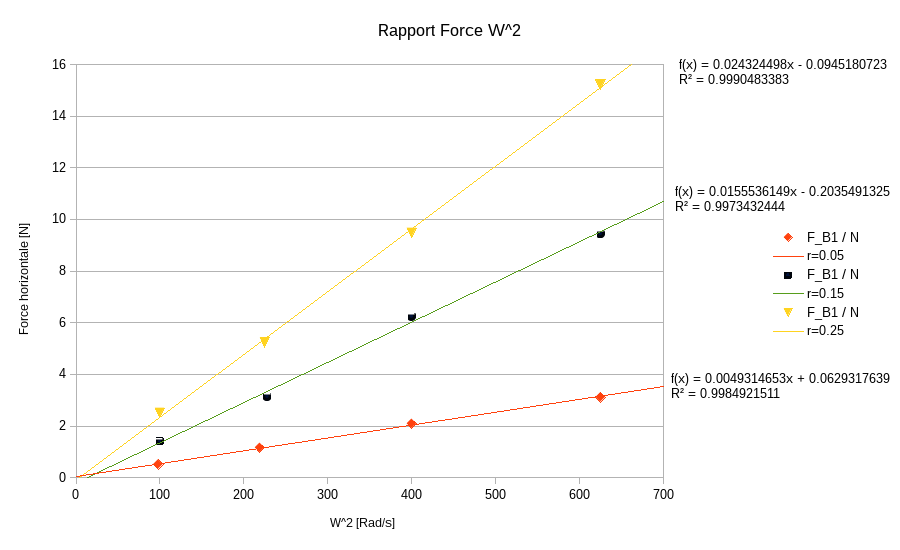
\includegraphics[height=25em]{Save03.png}
\end{figure}


\paragraph{Conclusion}

On peut donc raisonnablement affirmer que la force est linéairement proportionelle au carré de la vitesse angulaire.
Les droites extrapolées ne convergent pas toutes exactement vers l'origine, mais cette possiblité est incluse dans le calcul d'incertitudes.
